\documentclass{beamer}

\usepackage{amssymb,amsmath}
\usepackage{graphicx}
\usepackage{url}
\usepackage{color}
\usepackage{pagenote}[continuous,page]
\usepackage{relsize}		% For \smaller
\usepackage{url}			% For \url
\usepackage{epstopdf}	% Included EPS files automatically converted to PDF to include with pdflatex

%For MindMaps
% \usepackage{tikz}%
% \usetikzlibrary{mindmap,trees,arrows}%

%%% Color Definitions %%%%%%%%%%%%%%%%%%%%%%%%%%%%%%%%%%%%%%%%%%%%%%%%%%%%%%%%%
%\definecolor{bordercol}{RGB}{40,40,40}
%\definecolor{headercol1}{RGB}{186,215,230}
%\definecolor{headercol2}{RGB}{80,80,80}
%\definecolor{headerfontcol}{RGB}{0,0,0}
%\definecolor{boxcolor}{RGB}{186,215,230}

%%% Save space in lists. Use this after the opening of the list %%%%%%%%%%%%%%%%
%\newcommand{\compresslist}{
%	\setlength{\itemsep}{1pt}
%	\setlength{\parskip}{0pt}
%	\setlength{\parsep}{0pt}
%}

%\setbeameroption{show notes on top}

% You should run 'pdflatex' TWICE, because of TOC issues.

% Rename this file.  A common temptation for first-time slide makers
% is to name it something like ``my_talk.tex'' or
% ``john_doe_talk.tex'' or even ``discrete_math_seminar_talk.tex''.
% You really won't like any of these titles the second time you give a
% talk.  Try naming your tex file something more descriptive, like
% ``riemann_hypothesis_short_proof_talk.tex''.  Even better (in case
% you recycle 99% of a talk, but still want to change a little, and
% retain copies of each), how about
% ``riemann_hypothesis_short_proof_MIT-Colloquium.2000-01-01.tex''?

\mode<presentation>
{
  \usetheme{CambridgeUS}
  \usecolortheme{dolphin}
  \useoutertheme{default}
  \useinnertheme{default}
  \setbeamercovered{invisible} % or whatever (possibly just delete it)
}
\beamertemplatenavigationsymbolsempty

\usepackage[english]{babel}
%\usepackage[latin1]{inputenc}
\usepackage{subfigure}

\usepackage{times}
\usepackage[T1]{fontenc}
\usepackage{CJKutf8}

%% makes the ppagenote command for figure references at the end.
\makepagenote
\renewcommand{\notenumintext}[1]{}
\newcommand{\ppagenote}[1]{\pagenote[Page \insertframenumber]{#1}}

\title[Experiment Design (01CH740)]{Experiment Design for Computer Sciences (01CH740)}
\author[Claus Aranha]{Claus Aranha\\{\footnotesize caranha@cs.tsukuba.ac.jp}}
\institute[U. Tsukuba]{University of Tsukuba, Department of Computer Sciences}


\title[]{Experiment Design}
\subtitle[]{Lecture 1: Introduction}
\author[Claus Aranha]{Claus Aranha\\{\footnotesize caranha@cs.tsukuba.ac.jp}}
\institute{Department of Computer Science}

% This is being added to the footer and screwing things up
%\date{2015-04-14\\ \footnotesize{Last update \today}}


\begin{document}

\section{Introduction}
\subsection{Outline}

\begin{frame}
  \maketitle
\end{frame}

\subsection{Course Details}
\begin{frame}
  \frametitle{Course Goal}
  \begin{center}
    Understand how to design, execute and analyze an experiment, in a
    Computer Science context.
  \end{center}
  \bigskip

  {\small
  \begin{block}{Theoretical}
    \only<2>{
    What are the fundamentals of the Scientific method. How we
    recognize good/bad science, experiments, and scientific papers?
    Why are experiments necessary for our fields?}
  \end{block}
  \begin{block}{Instrumental}
    \only<3>{Statistical methods often used in an experimental context
      (hypothesis testing, significance, etc). How to analyse a data
      set. How to use the ``R'' tool to support statistical analysis
      of experiments.}
  \end{block}
  \begin{block}{Practical}
    \only<4>{How can I design an experiment for my own research? When I
      read other people's papers, can I spot and evaluate good/bad
      scientific practices? When considering a scientific hypothesis,
      or an engineering method, how to identify the assumptions of
      this research, and design experiments that test these
      assumptions or take them into account?}
  \end{block}}
\end{frame}

\begin{frame}
  \frametitle{This is a participative course}
  \begin{center}
    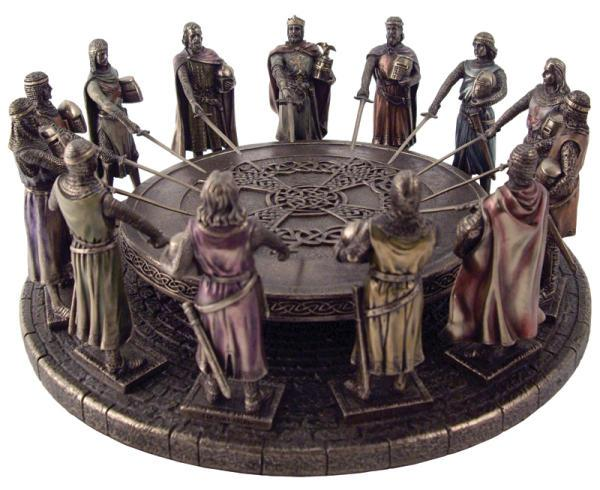
\includegraphics[width=0.4\textwidth]{img/roundtable}
  \end{center}
  \begin{block}{Rount table philosophy}
    Context (the reality of your research) is very important in the design of experiments. I will
    \structure{very often} ask you to give opinions based on your
    research experience!
  \end{block}
\end{frame}

\begin{frame}
  \frametitle{Outline}
  \begin{itemize}
  \item \structure{Class 1-2}: Introduction to Science and
    Experimentalism. Common good and bad practices in Science. Reflect
    on the meaning of research and how this influence your work.
  \item \structure{Class 3}: Basics of data handling: Understanding
    and visualizing data, simple statistics.
  \item \structure{Class 4}: Simple R-tutorial
    \medskip
  \item \structure{5/19 and 5/26}: \alert{No class}
    \medskip
  \item \structure{Class 5-9}: Techniques for experimental design,
    testing and analysis. Parameter selection. Hypothesis
    testing. Result evaluation.
  \item \structure{Class 10}: Report review.
  \end{itemize}
\end{frame}

\begin{frame}
  \frametitle{Evaluation} 

  Evaluation will be based on your ability to apply this classes ideas
  on your own research!

  \begin{description}
    {\small
  \item[Main Report]: Create an experimental design for your own
    research, using concepts introduced in this course. Define the
    factors, parameters, hypothesis, experiment and expected
    results. Use R to visually analyse your own data.

    \bigskip

  \item[Report on Good/Bad Science]: Write a review of two papers in
    your field of research (a good example, and a bad example). This
    review must be focused on the experimental design and analysis of
    the papers.  }
  \end{description}
  \vfill
  \begin{block}{}
    \begin{center}
      \alert{Just say NO to academic plagiarism}
    \end{center}
  \end{block}
\end{frame}

% Evaluation Methods

\subsection{Recommended Reading}
\begin{frame}
  \frametitle{Useful Materials -- Internet}
  
  \begin{itemize}
  \item \structure{Course
    Webpage}:\\\url{https://manaba.tsukuba.ac.jp/ct/course_397478}\\ Manaba
    Code: 7739931
  \item \structure{Lecture Notes
    (Github)}:\\\url{https://github.com/caranha/ExperimentDesignLectureNotes}
  \item \structure{Lecture Notes by Felipe
    Campelo}:\\\url{https://github.com/fcampelo/Design-and-Analysis-of-Experiments}
  \item \structure{R Programming
    Course}:\\\url{https://class.coursera.org/rprog-011}
  \end{itemize}
\end{frame}


\begin{frame}
  \frametitle{Useful Material -- Books}
  \begin{itemize}
  \item ``Experimental Methods for the Analysis of Optimization
    Algorithms'', Thomas Bartz-Beielstein et al.
  \item ``A Theoreticial Guide to the Experimental Analysis of
    Algorithms'', D.S. Johnson

    \medskip

  \item ``Introductory Statistics with R'', Peter Dalgaard
  \item ``Analysis of Categorical Data with R'', Christopher Bilder
    and Thomas M. Loughin
  \end{itemize}
\end{frame}
% Materials

\subsection{Self-Introduction}

\begin{frame}
  \frametitle{Let's get to know each other}
  \begin{itemize}
  \item What is your research area?
    \vfill
  \item What kind of experiments do you normally do?
    \vfill
  \item What is hard in your research area?
  \end{itemize}
\end{frame}

\section{What is Science?}
\subsection{Group Activities}
\begin{frame}
  \frametitle{What is Science?}
  \begin{center}
    {Give me your opinions!}
    \vfill
  \end{center}
\end{frame}

\begin{frame}
  \frametitle{The Science Game - Question}
  \begin{block}{}
    \begin{itemize}
    \item Imagine three numbers (triplets), and a rule behind them;
    \item Some triplets obey the rule, some don't;
    \item For example, the triplet ${3,6,9}$ obeys the rule!
    \end{itemize}
  \end{block}
  
  \begin{block}{Goal of the game:}
    \begin{itemize}
    \item Find out the secret rule for the triplets;
    \item To find the rule, you can ask the judge (me), if any trio of
      numbers obey the rule or not;
    \item Feel free to discuss among yourselves!
    \end{itemize}
  \end{block}
\end{frame}

\begin{frame}
  \frametitle{The Science Game - Answer}

  Did you find the rule?
  \begin{itemize}
    \item What rule did you find?
    \item How did you arrive on that rule?
    \item How certain are you that this is the secret rule?
  \end{itemize}
  \bigskip

  \begin{block}{The Rule}
    \only<2->{\structure{Three Real Numbers in increasing order.}}
  \end{block}
\end{frame}

\begin{frame}
  \frametitle{The Science Game - Insight}
  \begin{itemize}
  \item Each question was ``an experiment'';
  \item Did you use the experiments to confirm your idea, or to rule
    out other possibilities? (Confirmation Bias)
  \item What would be a good strategy for a similar game?
  \item When do you stop making questions?
  \end{itemize}
\end{frame}

\subsection{What is Science?}

\begin{frame}
  \frametitle{Hans, the Smart Horse}
  \begin{columns}[c]
    \column{0.3\textwidth} 
    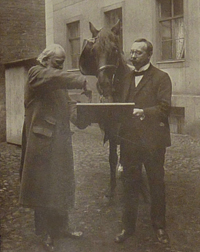
\includegraphics[width=\textwidth]{img/smarthorse}
    \column{0.7\textwidth} 
    Von Osten, the horse's trainer, displayed Hans amazing ability to
    do mathematical calculations by tapping his hoof.
  \end{columns}
  \medskip
  
  \begin{onlyenv}<2->
    \begin{block}{Oskar Pfungst's Experiments}
      \begin{itemize}
      \item Use people other than Van Osten to ask questions;
      \item<3-> Put people in different places;
      \item<4-> Make people ask questions they didn't know the answer;
      \end{itemize}
    \end{block}
  \end{onlyenv}
\end{frame}

\begin{frame}
  \frametitle{Common Misconceptions about Science}
  \begin{itemize}
  \item Science is a collection of facts;
  \item Science is the creation of new gadgets;
  \item Scientific ideas are absolute and unchangeable;
  \item Scientific ideas are subject to change, thus unreliable;
  \item Observation gives answers directly to the scientists;
  \item Science \structure{proves} stuff;
  \item Science can only \structure{disprove} things;
  \item The scientist works to \structure{show} his theory is right;
  \item Theory VS Law;
  \end{itemize}
\end{frame}

\begin{frame}
  \frametitle{The Scientific Method}
  \hfill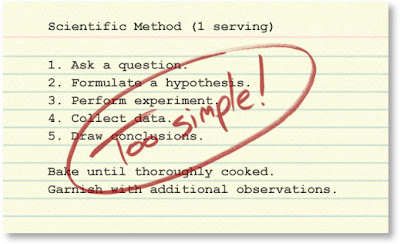
\includegraphics[width=0.6\textwidth]{img/recipe}\\
  \begin{itemize}
    \item A good start, but too simplified;
    \item The scientific method includes many iterations, interactions
      with multiple characters, etc;
    \item A set of \structure{principles}, not a set of
      \structure{rules}
  \end{itemize}
\end{frame}

\begin{frame}
  \frametitle{The Scientific Method}
  \begin{center}
    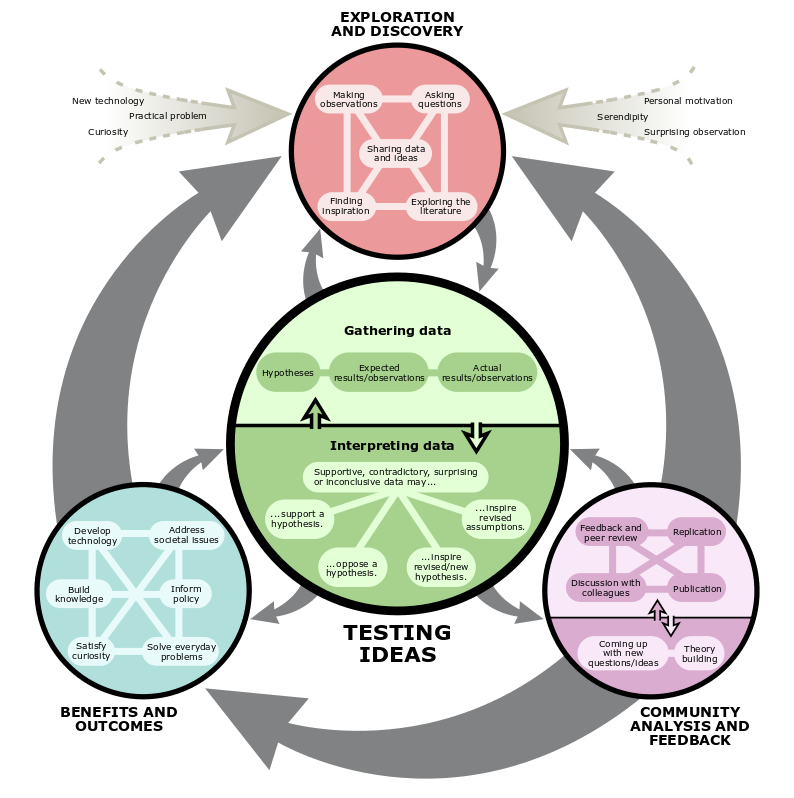
\includegraphics[height=.8\textheight]{img/understand}
  \end{center}
\end{frame}


\begin{frame}
  \frametitle{Important Considerations}
  \begin{itemize}
    \item Science is about collecting data (evidence) to understand a
      phenomenon -- but not hapzardly!
    \item ``Science is about being Wrong'' -- strive to look for
      evidence that the idea you hold is incorrect;
  \end{itemize}
\end{frame}

\begin{frame}
  \frametitle{The role of experimentation}
  \begin{columns}[c]
    \column{0.7\textwidth}
    \begin{itemize}
    \item In this sense, the \structure{experiment} is one of the main
      ways of collecting data;
    \item But before we get to the experiment, we will think about
      some questions you may have;
    \end{itemize}
    \column{0.3\textwidth}
    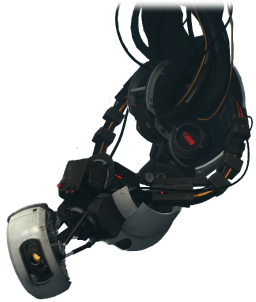
\includegraphics[width=0.9\textwidth]{img/glados.png}
  \end{columns}
\end{frame}

\section{Uncertainties}
\subsection{Uncertainties}
\begin{frame}
  \frametitle{Maybe Science is not for me...}
  \begin{block}{}
    \begin{columns}[c]
      \column{0.2\textwidth}
      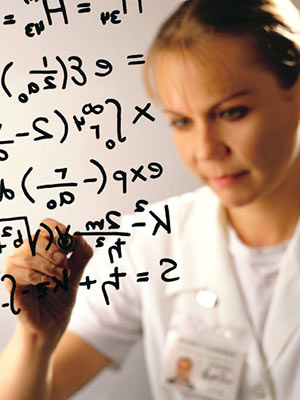
\includegraphics[width=1\textwidth]{img/mathematician}
      \column{0.8\textwidth} I don't really need experiments. All of
      my research involves well behaved, deterministic
      algorithms. Mathematical proofs are enough for me.
    \end{columns}
  \end{block}
  \begin{block}{}
    \begin{columns}[c]
      \column{0.8\textwidth} I don't really need experiments. My
      research involves creating a completely new service/device. If
      people seem excited about using this, then I'm doing it right.
      \column{0.2\textwidth}
      
\includegraphics[width=1\textwidth]{img/engineer}
    \end{columns}
  \end{block}
\end{frame}

\begin{frame}
  \frametitle{Uncertainties Everywhere} 

  When it comes to gathering data and experimental rigour, Researchers
  in Computer Science are still years behind other disciplines. A
  large disconnect still exists between the ``theorists'' and the
  ``empirists'' in CS.

  {\small
  \begin{block}{The Theorist's lament}
    Even if the algorithm is mathematically perfect, implementation
    details may affect the performance of the algorithm, or sometimes
    even the behavior. Many times, it is worth measurings the
    interaction betwee the system we are interested in, and other
    nsources.
  \end{block}
  \begin{block}{\hfill The Empirist's folly}
    Ad-hoc experiments hold many valuable lessons, but often they
    can't be used to get quantitatie information. Without care,
    uncertainties in the experiment may weaken the result.
  \end{block}}
\end{frame}

\begin{frame}
  \frametitle{Sources of Uncertainty}
  \begin{itemize}
  \item Physical Systems;
  \item Implementation Details;
  \item Random Number Generator;
  \item People in the experiment;
  \end{itemize}
\end{frame}

\begin{frame}
  \frametitle{Physical Systems}
  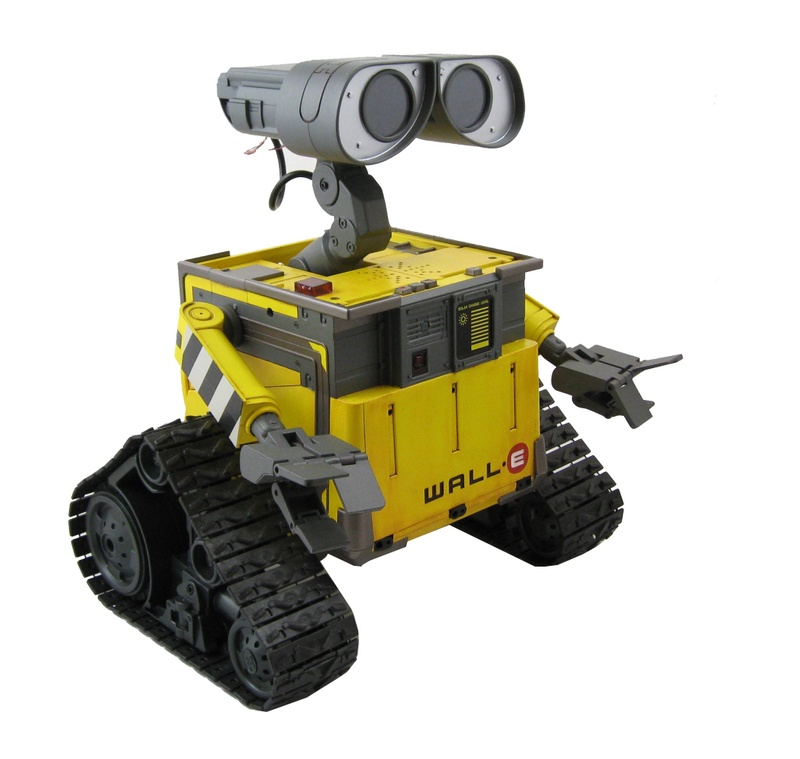
\includegraphics[width=0.3\textwidth]{img/robot}
  \begin{block}{}
    Transporting an algorithm from the blackboard to a production
    machine (or to a physical device) will include uncertainties from
    the interaction with the real world.
    \medskip
    (e.g.: Machine load, errors in robotic torque, etc)
  \end{block}
\end{frame}

\begin{frame}
  \frametitle{Implementation Details}
  \begin{block}{}
    Performance of an algorithm might vary greatly based:
    \begin{itemize}
    \item Programming techniques (data structures, design choices);
    \item Library used;
    \item Operating System;
    \item etc.
    \end{itemize}
  \end{block}
\end{frame}

\begin{frame}
  \frametitle{Random Number Generation}
  \begin{block}{}
    It is very difficult to prove an algorithmic behavior if part of
    it is defined by randomly generated numbers.
    \medskip
    
    Implementation of the RNG library can have a huge effect on
    algorithm behavior.
  \end{block}

  \hfill
  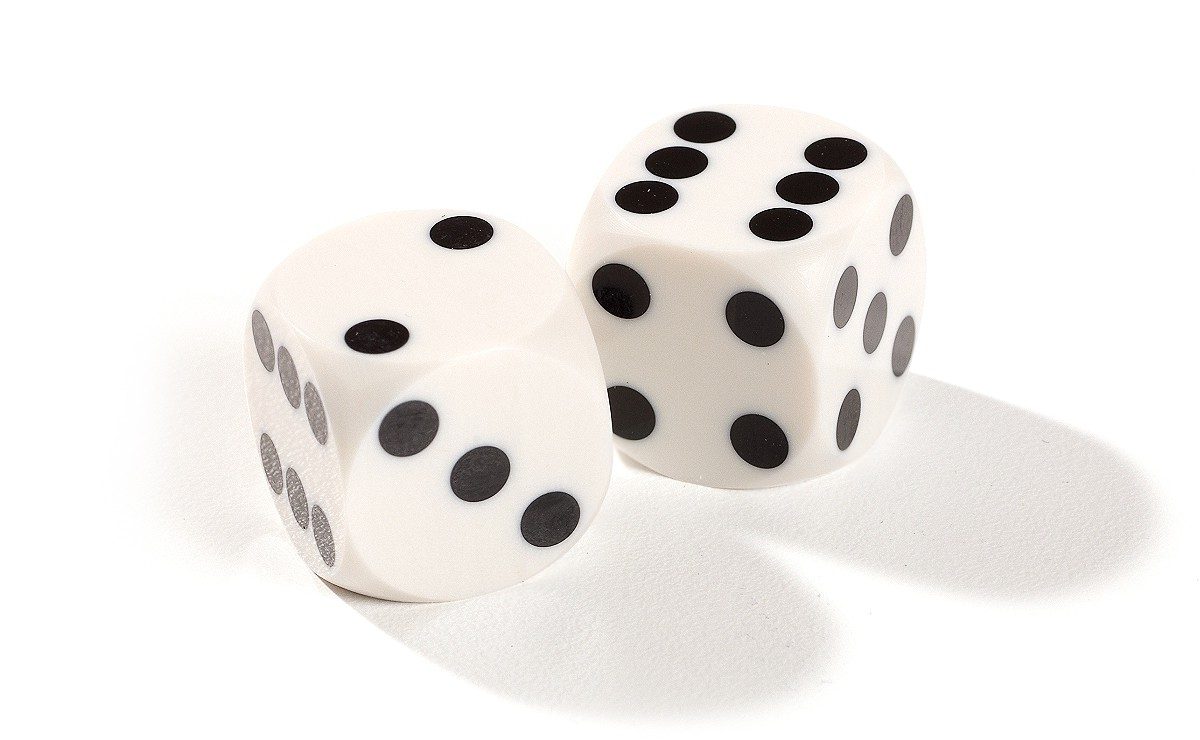
\includegraphics[width=0.4\textwidth]{img/dice}
\end{frame}

\begin{frame}
  \frametitle{Humans}
  \begin{block}{}
    Including humans in your research (eg. Interfaces), is a huge
    source of uncertainty regarding the results.
    \medskip
    
    You have to take into account not only how the humans will act,
    but also what are the characteristics of the particular group that
    you are using (don't do all your experiments on college students).
  \end{block}
\end{frame}

\begin{frame}
  \frametitle{Experiment Design} 

  By carefully designing the experimental methods of our research, we
  can account for these uncertainties in our results. 
  \bigskip
  \begin{itemize}
  \item Understand the influence of the uncertainty in the final results;\\
    or
  \item Take into account the state of the uncertainty as a condition
    for the experiment;
  \end{itemize}
\end{frame}

\begin{frame}
  \frametitle{Lack of an Experiment Design}
  \begin{columns}[c]
    \column{0.7\textwidth}
    \begin{block}{A common misunderstanding}
      Science is about creating cool gadgets and running many experiments.
    \end{block}
    \column{0.3\textwidth}
    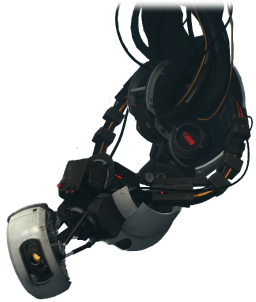
\includegraphics[width=0.9\textwidth]{img/glados.png}
  \end{columns}
  \vfill

  \begin{itemize}
  \item<2-> Experiments that only show the system works;\\
    {\small (of course it works, but WHY? And why is it good?)}
  \item<3-> Reinventing the wheel;\\ 
    {\small(Lack of comparisons and inspiration from other methods)}
  \item<4-> No knowledge is actually acquired;\\
    {\small(unreplicable papers, excess of data)}
  \end{itemize}
\end{frame}

\section{Experimental Practices} % Biggest section 

\subsection{Some examples of dealing with uncertainties}

\begin{frame}
  \frametitle{Experiment Design to the Rescue}
  \begin{center}
    How can we know if the effect we are observing is a result of the
    research being tested, or if it is an artifact from the
    uncertainties.
  \end{center}

%% For each uncertainty, give examples of how to deal with them 
%% In an experimental setting (uncertainty - dealing with them)
  \begin{onlyenv}<2>
    \begin{block}{Pshysical Uncertainties}
    \end{block}
  \end{onlyenv}
  \begin{onlyenv}<3> %% TODO
    \begin{block}{Implementation}
    \end{block}
  \end{onlyenv}
  \begin{onlyenv}<4> %% TODO
    \begin{block}{Random Numbers}
    \end{block}
  \end{onlyenv}
  \begin{onlyenv}<5> %% TODO
    \begin{block}{Human Factor}
    \end{block}
  \end{onlyenv}
\end{frame}

\subsection{Good Experiments, Bad Experiments}

\begin{frame}
  \frametitle{Goals for an experiment}
  
  The main characteristics that we look for in a good experiment are:
  \bigskip 

  \begin{columns}[c]
    \column{0.8\textwidth}
    {\small
      \begin{enumerate}
      \item [Clarity:] Does the experiment really show the kind of
        information that we are interested in? Can it be used to confirm
        or reject our hypothesis? Does it show any other interesting data?
      \item [Replicability:] Can other people repeat my experiment 5, 10
        years in the future? Are all algorithms, parameters and data well
        defined? Am I sharing my source code?
      \item [Control:] How many ``moving wheels'' and ``conditions'' does
        my experiment has? Do I know how general the results obtained are?
    \end{enumerate}}
  \end{columns}
\end{frame}

\begin{frame}
  \frametitle{On experiments}
  \vfill
  \begin{block}{}
    \begin{columns}[c]
      \column{0.8\textwidth} 
      {\footnotesize {\it``However, experiments require a lot of
      work, so the reader may be warned: performing a good experiment
      is as demanding as proving a new theorem.''}\\
      -- Hans-Paul Schwefel}
      \column{0.1\textwidth}
      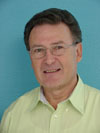
\includegraphics[width=1\textwidth]{img/schwefel}
    \end{columns}
  \end{block}
\end{frame}

\begin{frame}
  \frametitle{Experiment Design: Control} %% TODO: 

  \begin{itemize}
  \item Decide what is the quantity to be examined;
  \item Control the values of all other quantities;
  \item Define the range and index for the variation;
  \end{itemize}
  \begin{block}{}
    There are principles and rules for defining these designs, which
    we will watch carefully in the next class.
  \end{block}
\end{frame}

\begin{frame}
  \frametitle{Experiment Design: Replicability} %% TODO: finish this
  \begin{itemize}
  \item If other people follow our steps, can they reach the same
    results as we did?
  \item Extremely important not only for validation, but also for
    other people to use your research;
  \item Make data, parameters and source code available;
  \item Take special care with small tricks and hacks that you may
    have added during your work;
  \end{itemize}
\end{frame}

\begin{frame}
  \frametitle{Experiment Design: Clarity} %% TODO: finish this
  \begin{itemize}
  \item Besides clarity regarding the replicability of your research,
    clarity regarding the scope and achievements of your work are
    important;
  \item In which cases is your research valid?
  \item What are your assumptions?
  \end{itemize}
  \bigskip

  \begin{block}{What are the assumptions made?}
    A very narrow claim with clear assumptions is better than a wide
    claim that does not state its assumptions.
  \end{block}
\end{frame}

\subsection{Bad practices}
%%% The ugly
\begin{frame}
  \frametitle{Experiments: The Ugly}
  \begin{block}{}
    News link:
    ``\href{http://www.newscientist.com/article/mg21528826.000-is-medical-science-built-on-shaky-foundations.html}{Two
      thirds of drug studies failed to replicate}''
  \end{block}
  \bigskip
  
  \begin{itemize}
  \item Not all data available;
  \item Not all experimental parameters available;
  \item Some details of the experimental method were not listed
    (hacks)
  \end{itemize}
  \vfill
  \begin{center}
    (Specially bad in the computer sciences)
  \end{center}
  
\end{frame}



\begin{frame}
  \frametitle{Bad Practices}

  \begin{block}{Careless Experimentation}

    \begin{columns}[c]
      \column{0.7\textwidth} 
      \smaller{``To Consult the statician after an experiment is finished is
      often merely to ask him to conduct a post mortem examination. He
      can perhaps say what the experiment died of.'' -- Sir Ronald Fischer}
      \column{0.20\textwidth}
      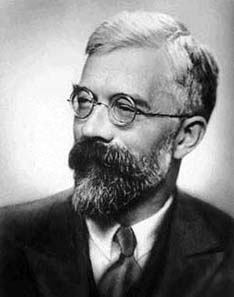
\includegraphics[width=0.5\textwidth]{img/fisher}
    \end{columns}

    \medskip

    \begin{itemize}
      \item People are well meaning (I hope!), but sloppy research
        still gets done.
        \smallskip

      \item<2-> Lack of training, Lack of awareness, Publication bias;
        \smallskip

      \item<3-> Correct Goal: Finding out the truth;
      \item<3-> Common Goal: Finding out that the algorithm is
        publishable;
        \smallskip
    \end{itemize}
  \end{block}
\end{frame}

\begin{frame}
  \frametitle{Careless Experimentation}
  
  \begin{block}{}
    ``The presented results represent the average from 30 runs of each
    algorithm''
  \end{block}

  \begin{onlyenv}<2>
  \begin{block}{What ``average of 30 runs'' does not say}
    \begin{columns}[c]
      \column{0.45\textwidth}
      {\bf Proposed Algorithm}
      \medskip

      \begin{itemize}
        \smaller{
      \item Careful implementation and error checking;
      \item Exhaustive search of appropriate parameters;
      \item Many Experimental runs;}
      \end{itemize}
      \column{0.45\textwidth}
      {\bf Comparison Algorithm}
      \medskip

      \begin{itemize}
        \smaller{
      \item Careless implementation: Good enough if it runs;
      \item Parameters found in the literature;
      \item Single experimental run;}
      \end{itemize}
    \end{columns}
  \end{block}    
  \end{onlyenv}
\end{frame}

\begin{frame}
  \frametitle{Careless Experimentation}
  \begin{block}{Other Common Problems}
    \begin{itemize}
    \item No clear definition of the Goal of the experiment (confusion
      among hypothesis, theory, explanation, conjecture)
      \smallskip

    \item Cherry picking of data/results (This data that does not work
      falls outside the scope of this paper).
      \smallskip

    \item Personal Biases (getting experimentation backwards: trying
      to show that one method {\bf is} better, instead of
      investigating {\bf if} the method is better).
    \end{itemize}
  \end{block}
\end{frame}

\begin{frame}
\frametitle{Careless Experimentation}
\begin{center}
  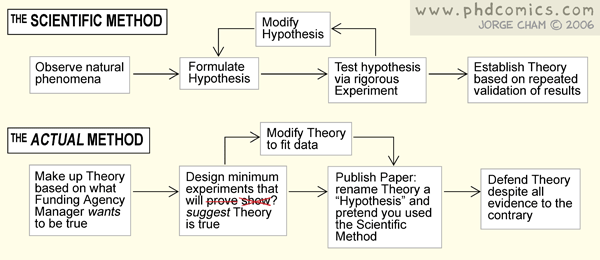
\includegraphics[width=1\textwidth]{img/phdcomics}
\end{center}
\end{frame}

\begin{frame}
  \frametitle{Other common mistakes}
  \begin{block}{Premature conclusions}
    \begin{itemize}
    \item Stop as soon as a successful result is achieved;
    \item No random repetitions, no stress tests;
    \item Even some negative results can be informative!
    \end{itemize}
  \end{block}
\end{frame}




% Cargo cult science

% Of course, there are the bad experiments that are in this way
% because of nefarious reasons. But I want to imagine that this is not
% our case.

\section{Conclusion}
\subsection{conclusion}

\begin{frame}
  \frametitle{Conclusion} Rigorous scientific methods are important
  for computer science, in order to isolate uncertainties and quantify
  our discoveries.
\end{frame}

\begin{frame}
  \frametitle{For the Next Class}
  \begin{itemize}
    \item Each of you should prepare a new short introduction to your
      disciplines/research topic;
    \item Take into account the topics discussed today;
    \item How would you apply this knowledge to your existing
      research;
  \end{itemize}
\end{frame}


\begin{frame}
  \frametitle{One final message}
  \begin{block}{}
    It is important to be literate in the scientific method, not only
    for your own research's sake. We are also agents of change in the
    population and, as such, we need to be aware of good and bad
    science, and able to point the difference to the society.
  \end{block}
\end{frame}

\begin{frame}
  \frametitle{Acknowledgements}
  \begin{itemize}
  \item Felipe Campelo, for many comments and insights on the contents of this course;
  \item ``The Science Game'' inspired from \url{http://hpmor.com};
  \item ``Common Misconceptions About Science'' \url{http://undsci.berkeley.edu/teaching/misconceptions.php}
  \end{itemize}
\end{frame}

\begin{frame}
  \frametitle{Contact Me!}
  \begin{description}
    \item[E-mail:] caranha\@@cs.tsukuba.ac.jp
    \item[Homepage:] \url{http://conclave.cs.tsukuba.ac.jp}
    \item[Twitter:] @caranha
  \end{description}
\end{frame}

\end{document}
